\documentclass{beamer}

\usepackage{centernot}
\usepackage{amsmath, amssymb, graphics, setspace}

\title{From Zero to RAPIDS in 7 Days: \\
       Learning How to Use RAPIDS for Data Science on Comet}
\author{Marty Kandes \\
   Computational \& Data Science Research Specialist
   High-Performance Computing User Services Group \\ 
   San Diego Supercomputer Center \\
   University of California, San Diego}
\date{NVIDIA Deep Learning Institute @ SDSC \\
   Wednesday, August 21st 2019 \\
   1:00PM - 2:30PM PT}

\begin{document}
\maketitle

\begin{frame}
   \frametitle{About Me}
   \begin{itemize}
      \setlength\itemsep{1.5em}
      \item High-Performance Computing Group @ SDSC
      \item Distributed High-Throughput Computing Group @ SDSC
      \item Computational Science Research Center @ SDSU
      \item I am most definitely \textbf{not} a data science expert
   \end{itemize}
\end{frame}

\begin{frame}
   \frametitle{About You}
   \LARGE
   Who are you?
\end{frame}

\begin{frame}
   \frametitle{Question 1}
   \LARGE
   Are you a graduate student, post-doctoral scholar, research staff member, or professor at UCSD (or another UC campus?
\end{frame}

\begin{frame}
   \frametitle{Question 2}
   \LARGE
   Are you a graduate student, post-doctoral scholar, research staff member, or professor at a non-UC U.S. educational institution (or another non-profit research entity?)
\end{frame}

\begin{frame}
   \frametitle{Question 3}
   \LARGE
   Are you an industry partner?
\end{frame}

\begin{frame}
   \frametitle{Question 4}
   \LARGE
   Do you have a (non-training) user account on Comet or TSCC?
\end{frame}

\begin{frame}
   \frametitle{Question 5}
   \LARGE
   Does your day-to-day research work involve data science?
\end{frame}

\begin{frame}
   \frametitle{Question 6}
   \LARGE
   What programming languages do you use day-to-day for your research?
\end{frame}

\begin{frame}
   \frametitle{Question 7}
   \LARGE
   Do you use NVIDIA GPUs in your day-to-day research work?
\end{frame}

\begin{frame}
   \frametitle{Question 8}
   \LARGE
   Have you ever run your own website?
\end{frame}

\begin{frame}
   \frametitle{Question 9}
   \begin{figure}[htbp]
      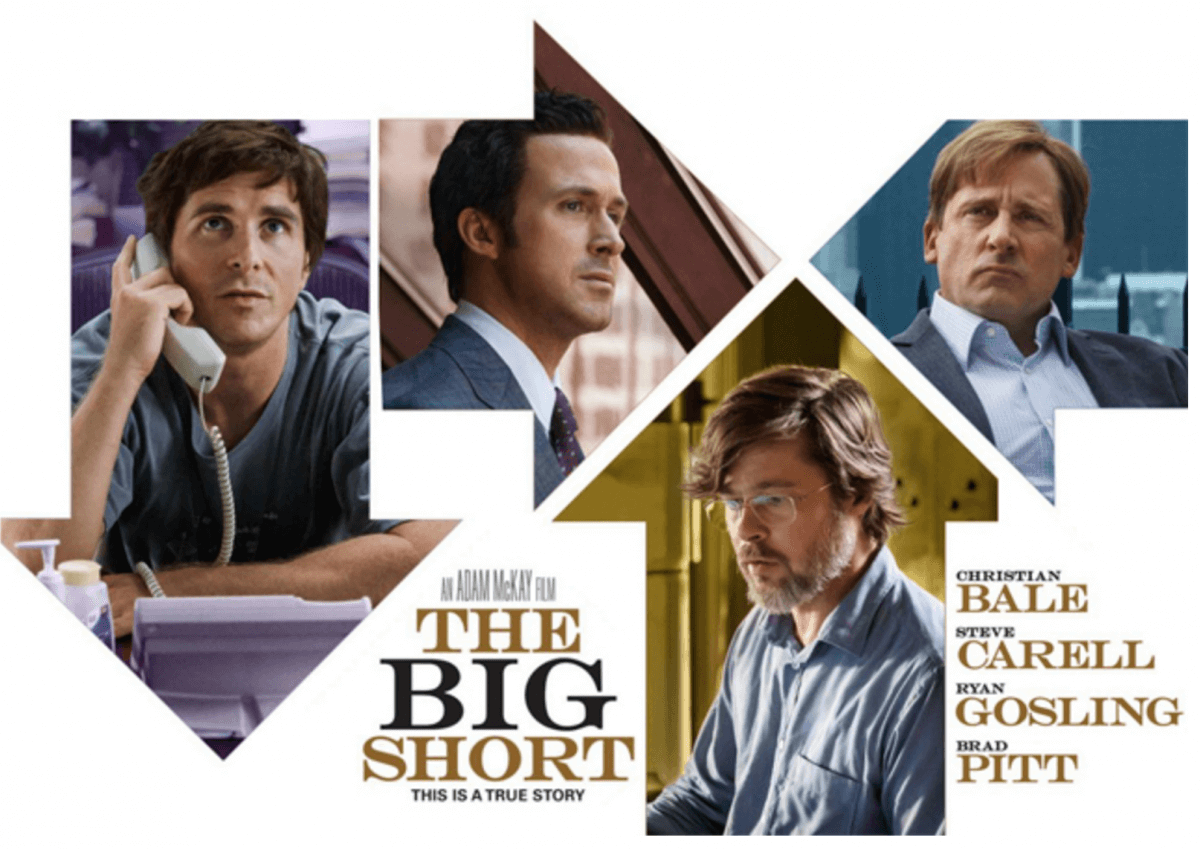
\includegraphics[width=0.7\textwidth]{images/THE-BIG-SHORT-2-1200x849.png}
   \end{figure}
   \begin{center}\LARGE
      Have you seen this movie?
   \end{center}
\end{frame}

\begin{frame}
   \frametitle{An Overview: From Zero to RAPIDS in 7 Days}
   \begin{itemize}
      \setlength\itemsep{1.0em}
      \item How to access supercomputing resources for your research 
      \item A (very) quick, historical note on Data Science
      \item How to monitor your CPU/GPU resources
      \item How to run a Jupyter Notebook
      \item How to use Pandas
      \item More than you probably wanted to know about the Fannie Mae Single-Family Loan Performance Dataset (or How I Learned to Stop Worrying about the Performance Data and Love the Acquisition Data)
      \item How to accelerate your Pandas-like workflows with cuDF
   \end{itemize}   
\end{frame}

\begin{frame}
   \frametitle{A not-so long time ago in a data center not that far, \\
               far away ...}
   \begin{itemize}
      \setlength\itemsep{1.0em}
      \item In 2012, 99\% of all computational jobs run on NSF-funded
         HPC resources utilized fewer than 2048 CPU-cores, while
         accounting for approximately 50\% of the total core-hours
         consumed across these resources.
      \item Nearly 70\% of all jobs actually ran on only a single
         compute node (16 CPU-cores) or less.
   \end{itemize}
\end{frame}

\begin{frame}
   \frametitle{Comet: A Supercomputer Built to Serve the 99\%}
   \vspace{-1.0em}
   \begin{figure}[htbp]
      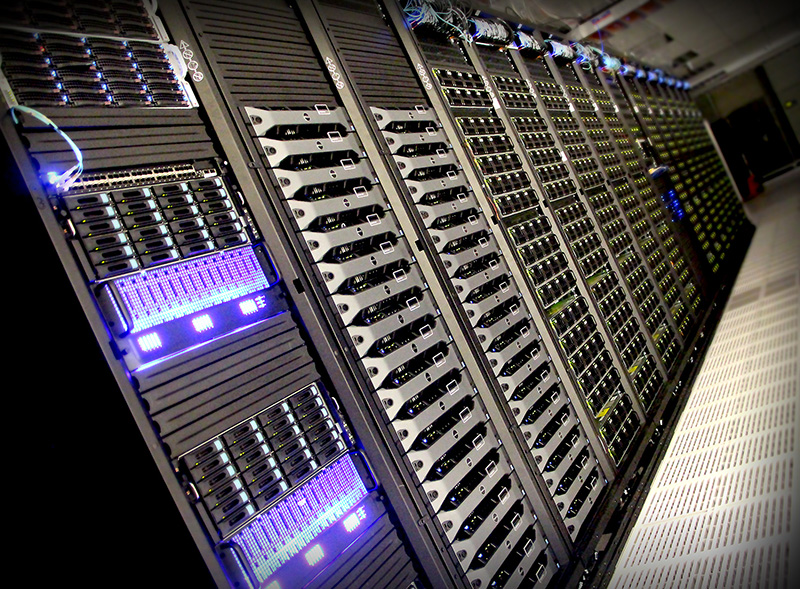
\includegraphics[width=0.9\textwidth]{images/comet.jpg}
   \end{figure}
\end{frame}

\begin{frame}
   \frametitle{Comet By the Numbers}
   \begin{itemize}
      \small
      \setlength\itemsep{1.0em}
      \item \textbf{1944 compute nodes}: Dual-socket; 2.5 GHz Intel Xeon
         E5-2680v3 processors; 12 cores per processor; 128 GB DDR4 DRAM;
         120 GB/s memory bandwidth; 320 GB SSD (210 GB Avail)
      \item \textbf{4 large-shared memory nodes}: Quad-socket; 2.2 GHz
         Intel Xeon E7-8860v3 processors; 16 cores per processor; 1.5 TB
         DDR4 DRAM; 400 GB SSD (260 GB Avail)
      \item \textbf{36 k80 gpu nodes}: Same as standard
         \textit{compute} node, but with 2 PCIe-based NVIDIA Tesla K80
         dual-GPU accelerators per node
      \item \textbf{36 p100 gpu nodes}: Dual-socket; 2.4 GHz Intel Xeon
         E5-2680v4 processors; 14 cores per processor; 128 GB DDR4 DRAM;
         150 GB/s memory bandwidth; 400 GB SSD (260 GB Avail);  4
         PCIe-based NVIDIA Tesla P100 GPU accelerators per node
   \end{itemize}
   \begin{center}
      \textbf{2.76 Pflop/s}
   \end{center}
\end{frame}

\begin{frame}
   \frametitle{Comet By the Numbers}
   \begin{itemize}
      \small
      \setlength\itemsep{1.0em}
      \item \textbf{Interconnect}: Mellanox FDR (56Gbps) InfiniBand;
         hybrid fat-tree topology; rack-level (72 node) full bisection
         bandwidth; 4:1 over-subscription cross-rack bandwidth
      \item \textbf{Storage}: NSF-based \$HOME storage (100 GB per
         user; \textcolor{green}{weekly backups}); 6.4 PB 200 GB/s
         Lustre-based parallel filesystem storage (intermediate-term
         use: at least 500 GB per group allocation in /oasis/projects;
         short-term use: up to 10 TB per user in /oasis/scratch;
         \textit{2M inodes limit}; \textcolor{red}{NO BACKUP!})
      \item \textbf{Applications}: More than 173 software applications
         and libraries maintained and deployed via Rocks (Linux) cluster
         distribution; accessible to users via software modules; span a
         wide range of scientific disciplines, including, but not
         limited to, bioinformatics, chemistry, data analytics,
         engineering, fluid dynamics, mathematics, molecular dynamics,
         neuroscience, and statistics
      \item \textbf{Scientific Impact}: 1755 PIs; 358 institutions;
         1144 research allocations; 4709 direct-access users; 33000+
         gateway users; 997 publications
   \end{itemize}
\end{frame}

\begin{frame}
   \frametitle{Computing Without Boundaries}
   \vspace{-1.0em}
   \begin{figure}[htbp]
      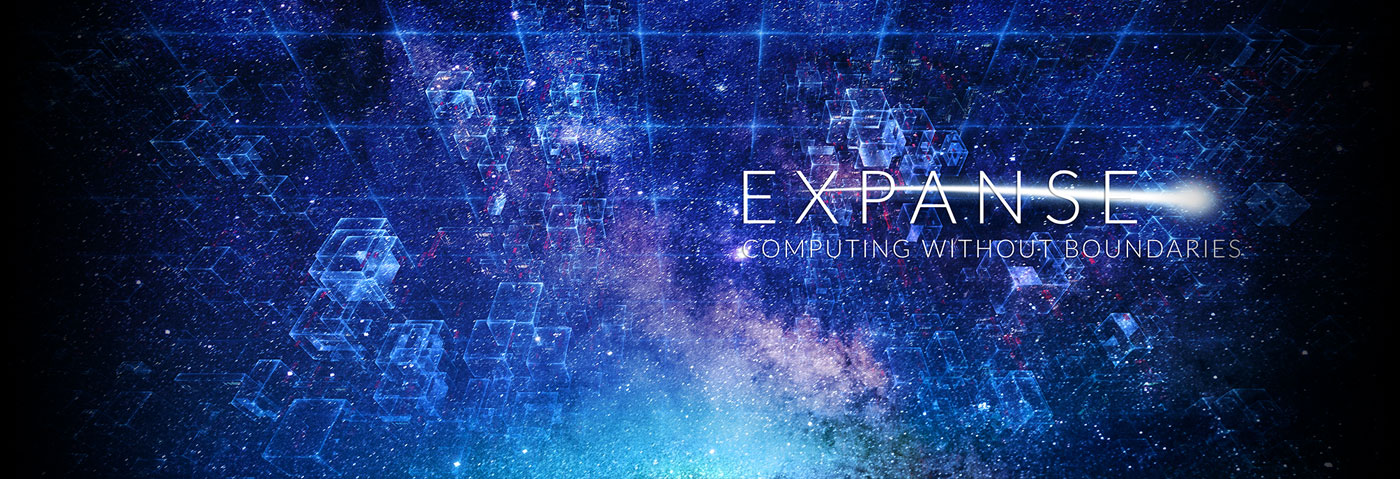
\includegraphics[width=1.0\textwidth]{images/expanse-banner.jpg}
   \end{figure}
   \begin{center}
      Coming September 2020
   \end{center}
\end{frame}

\begin{frame}
   \frametitle{Triton Shared Compute Cluster (TSCC)}
   \begin{itemize}
      \setlength\itemsep{1.0em}
      \item Medium-scale research cluster (launched in 2013)
      \item Hybrid business model:
      \begin{enumerate}
         \vspace{0.5em}
         \item ``condo'' (buy-in)
         \item ``hotel'' (pay-as-you-go)
      \end{enumerate}
      \item Mixed architecture: 375 CPU nodes (7k cores); 50 GPU nodes (300 GPUs); 850 TB parallel filesystem; Ethernet + Infiniband networks
      \item Approximately 30 participating labs/research groups
   \end{itemize}
\end{frame}

\begin{frame}
   \frametitle{How do I get time on Comet or TSCC?}
   \begin{itemize}\setlength\itemsep{1.5em}
      \item Comet:
         \vspace{0.5em}
         \begin{enumerate}\setlength\itemsep{1.5em}
            \item UC: HPC @ UC Program - \url{https://www.sdsc.edu/collaborate/hpc\_at\_uc.html} 
            \item UC/Non-UC/Non-Profit: XSEDE - \url{https://www.xsede.org/} 
            \item Industry: Ron Hawkins @ SDSC, Industry Relations
         \end{enumerate}
      \ \\ \ \\
      \item TSCC:
         \vspace{0.5em}
         \begin{enumerate}\setlength\itemsep{1.5em}
            \item UC/Non-UC/Non-Profit/Industry: Ron Hawkins @ SDSC, Industry Relations
         \end{enumerate}
   \end{itemize}
\end{frame}

\begin{frame}
   In the beginning (of Data Science) ...
\end{frame}

\begin{frame}
   \frametitle{Mid-1980s - Today} 
   \begin{columns}
      \begin{column}{0.5\textwidth}
         \begin{figure}[htbp]
            
\includegraphics[width=1.0\textwidth]{images/Excel_97.png}
         \end{figure}
      \end{column}
      \hfill
      \begin{column}{0.5\textwidth}
         \begin{figure}[htbp]
            
\includegraphics[width=1.0\textwidth]{images/bill-excels.jpg}
         \end{figure}
      \end{column}
   \end{columns}
\end{frame}

\begin{frame}
   \frametitle{3200-3000 BCE}
   \begin{columns}
      \begin{column}{0.7\textwidth}
         \begin{figure}[htbp]
            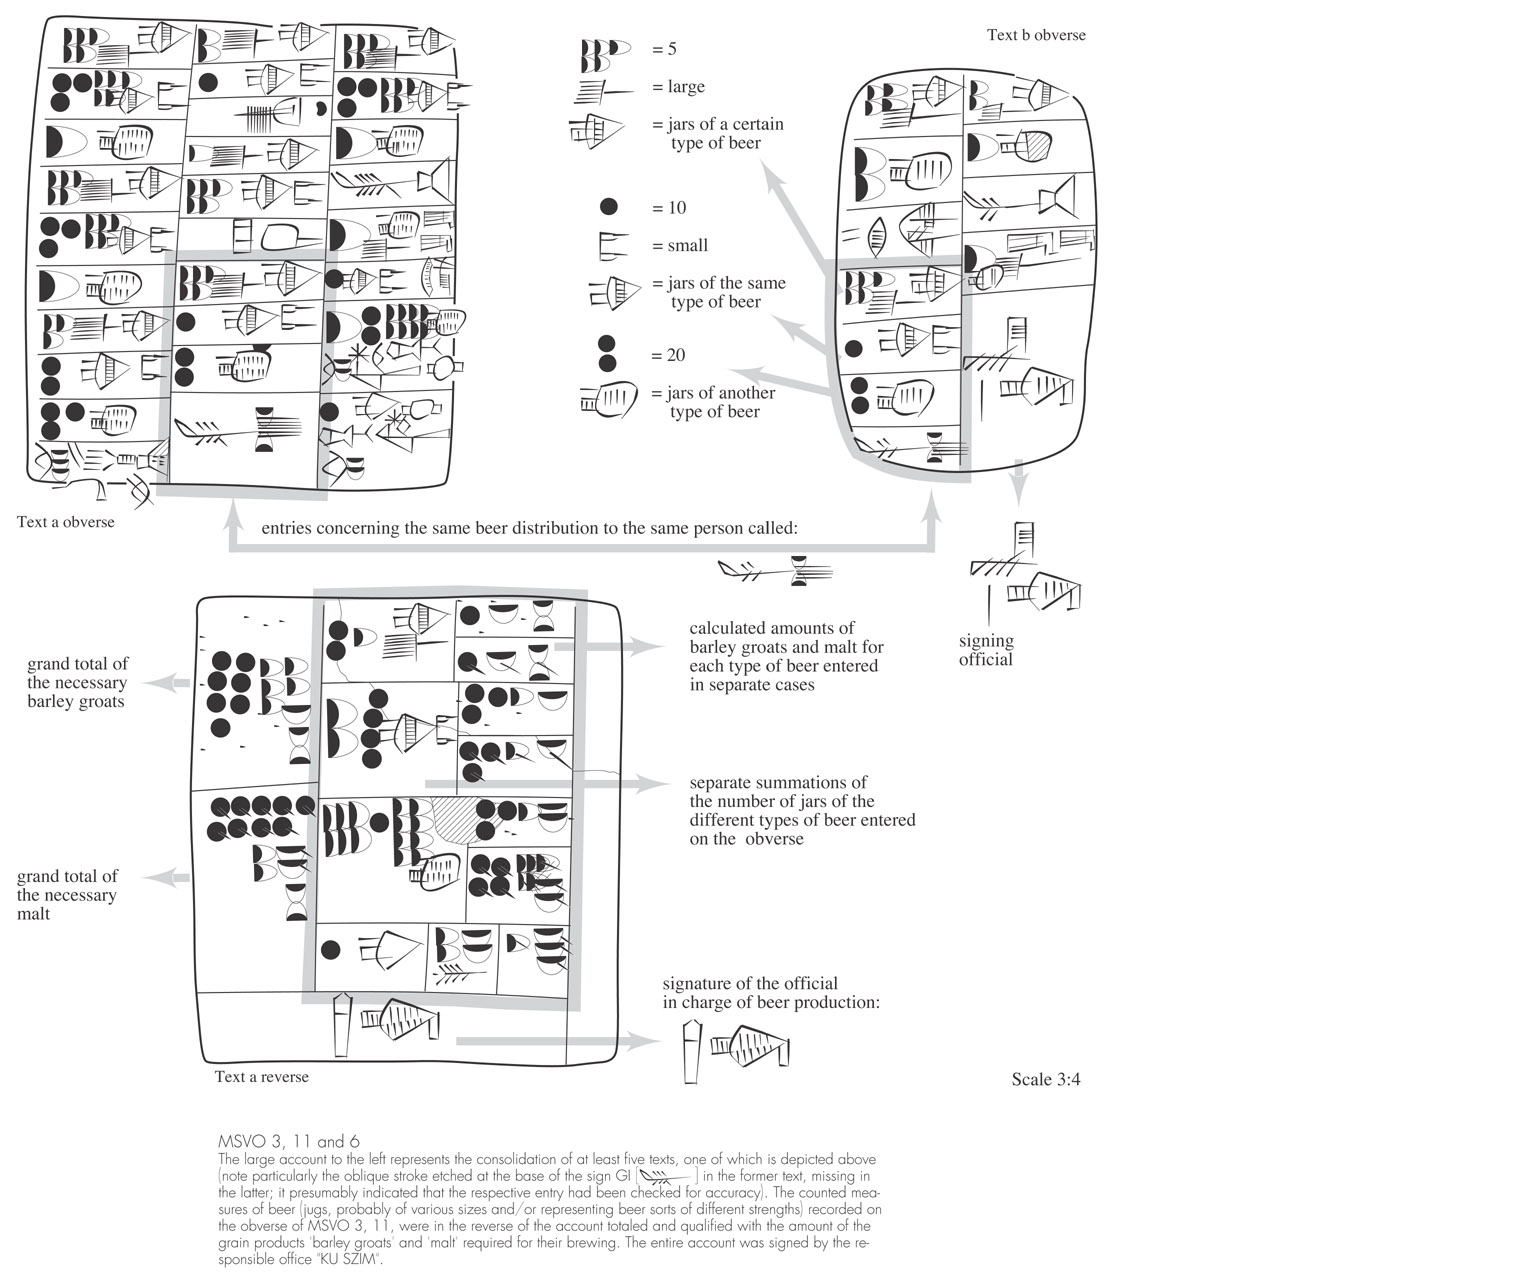
\includegraphics[width=1.0\textwidth]{images/P005322_ld.jpg}
         \end{figure}
      \end{column}
      \hfill
      \begin{column}{0.4\textwidth}
         \begin{figure}[htbp]
            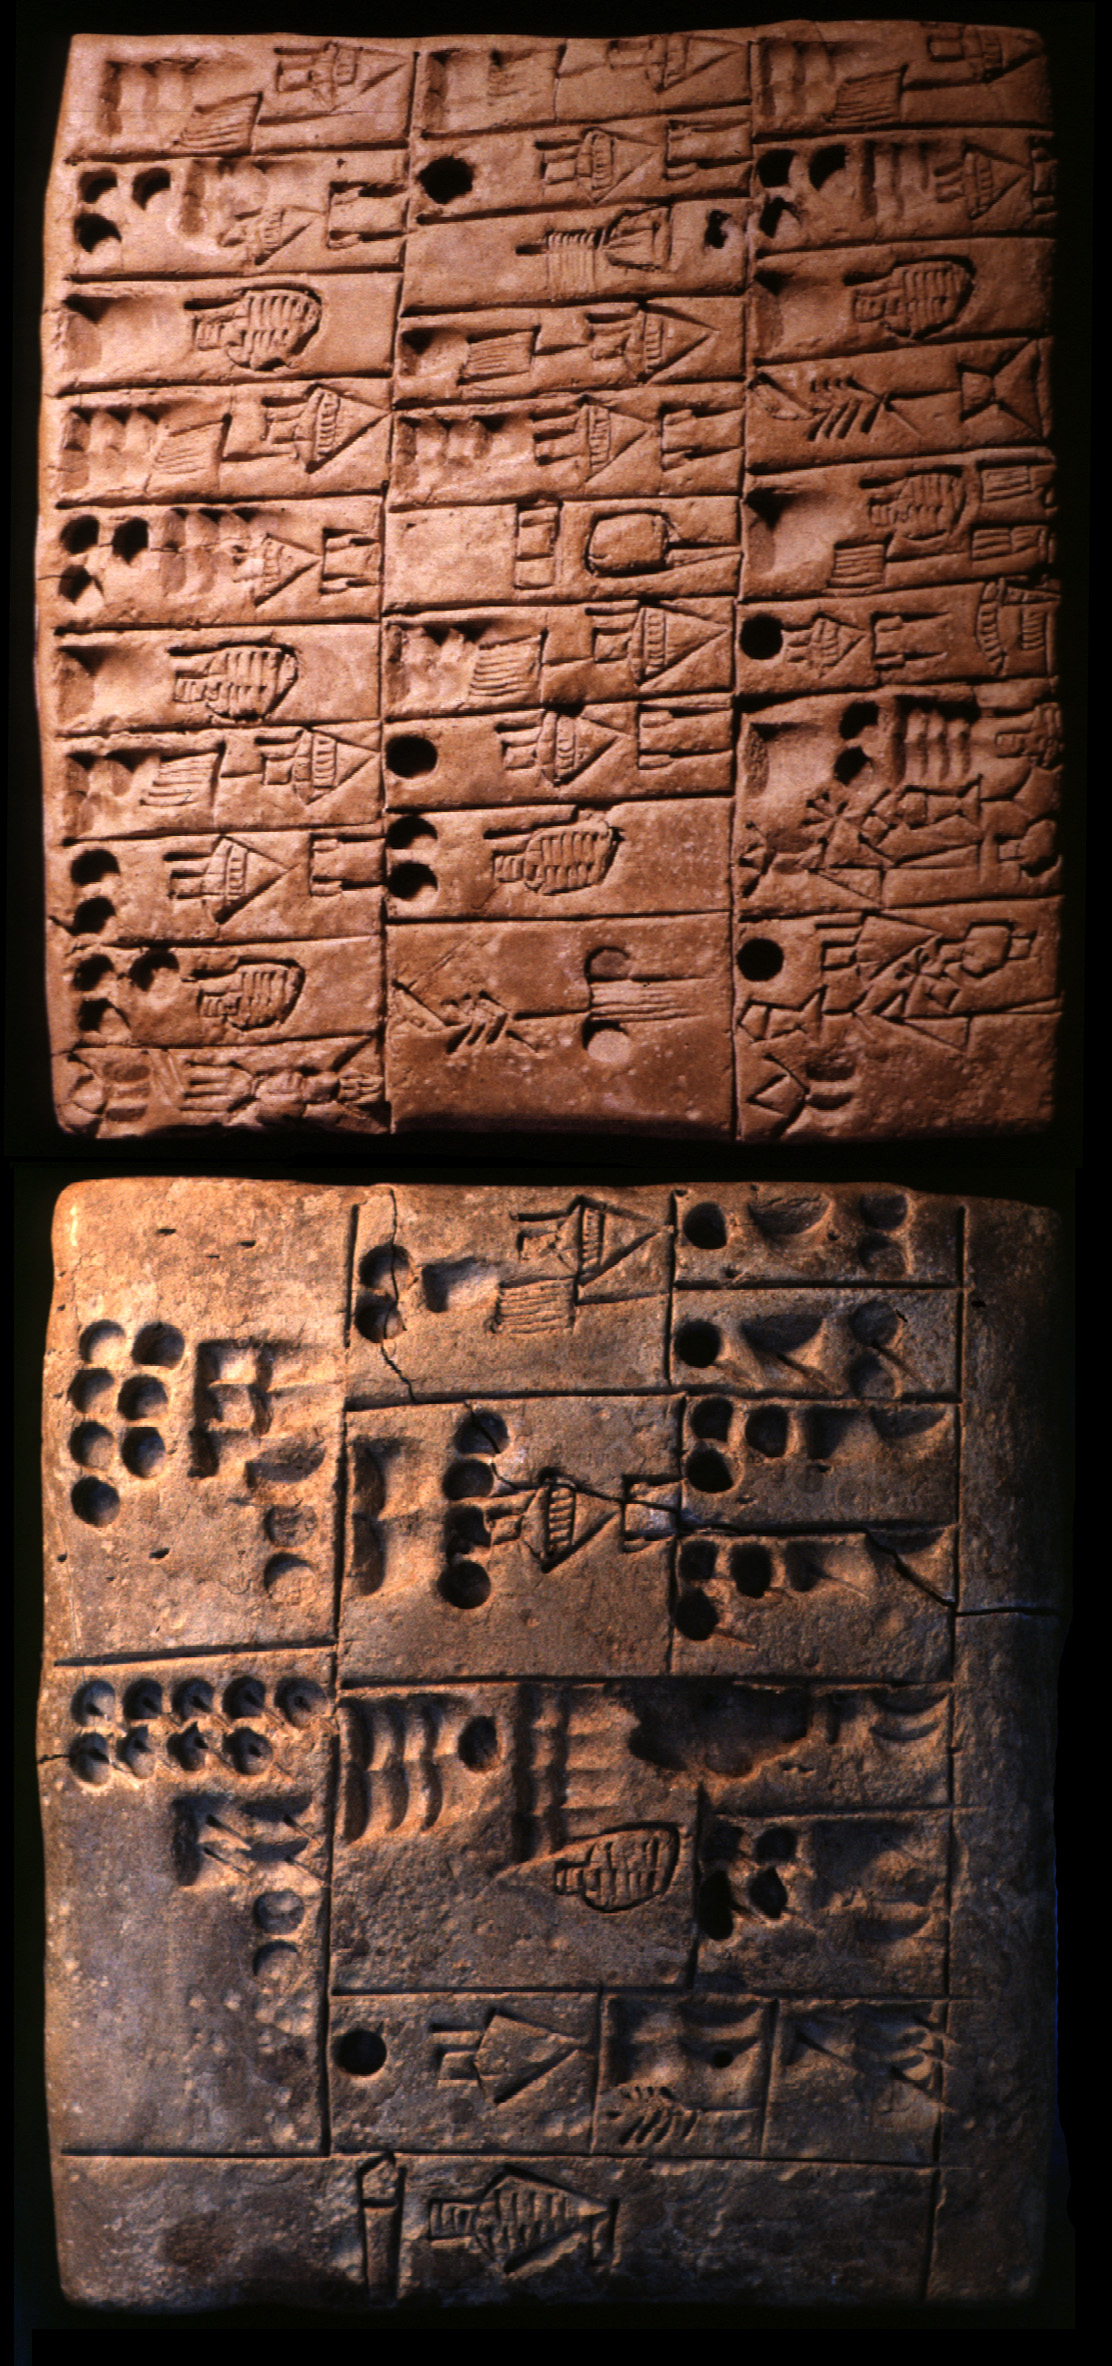
\includegraphics[width=0.7\textwidth]{images/P005322.jpg}
         \end{figure}
      \end{column}
   \end{columns}
\end{frame}

\begin{frame}
   \frametitle{Today}
   \begin{tabular}{cc}
      
\includegraphics[width=0.1\textwidth]{images/2000px-Microsoft_Office_Excel_2018_present.png} &
      
\includegraphics[width=0.3\textwidth]{images/Apache_Spark_logo.png} \\
      
\includegraphics[width=0.3\textwidth]{images/hadoop_logo.jpeg} &
      
\includegraphics[width=0.2\textwidth]{images/r_logo.jpg} \\
      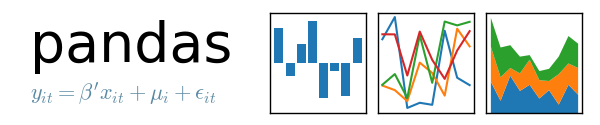
\includegraphics[width=0.5\textwidth]{images/pandas_logo.png} &
      
\includegraphics[width=0.4\textwidth]{images/rapids_logo.png}
   \end{tabular}
\end{frame}

\end{document}
